\documentclass{article}
\usepackage{geometry}
\usepackage{parskip}


\title{Outlier/Anomaly Detection}
\author{Dr. M. Kamakshaiah}

\usepackage{Sweave}
\begin{document}
\Sconcordance{concordance:outliers.tex:outliers.Rnw:%
1 8 1 1 0 17 1 1 2 1 0 2 1 4 0 1 2 6 1 1 33 35 0 1 2 5 1 1 2 1 0 2 1 7 %
0 1 2 2 1 1 2 1 0 1 1 11 0 1 2 6 1 1 2 1 0 2 1 4 0 1 2 5 1}

\maketitle 
\newpage
\tableofcontents
\newpage
\section{What is Outlier}

In statistics, an outlier is an observation point that is distant from other observations. An outlier may be due to variability in the measurement or it may indicate experimental error; the latter are sometimes excluded from the data set. An outlier can cause serious problems in statistical analyses. \footnote{https://en.wikipedia.org/wiki/Outlier}

In the case of normally distributed data, the three sigma rule means that roughly 1 in 22 observations will differ by twice the standard deviation or more from the mean, and 1 in 370 will deviate by three times the standard deviation. In a sample of 1000 observations, the presence of up to five observations deviating from the mean by more than three times the standard deviation is within the range of what can be expected, being less than twice the expected number and hence within 1 standard deviation of the expected number and not indicate an anomaly. 

\subsection{Manual Approach}

Usually outliers are understood with respect to Confidence Intervals (CI) where significance is $1-ci$ also known as $\alpha$. For instance, if we assume a normal distribution, then the outliers are determined based on $\mu \pm n.\sigma$, where $n$ is the scale e.g. 1, 2, 3 $\cdots$   

\subsubsection{R Code}

\begin{Schunk}
\begin{Sinput}
> x <- abs(round(rnorm(100), 2))
> par(mfrow = c(1, 2))
> plot(x); hist(x, freq = FALSE); lines(density(x), col = "red")
\end{Sinput}
\end{Schunk}
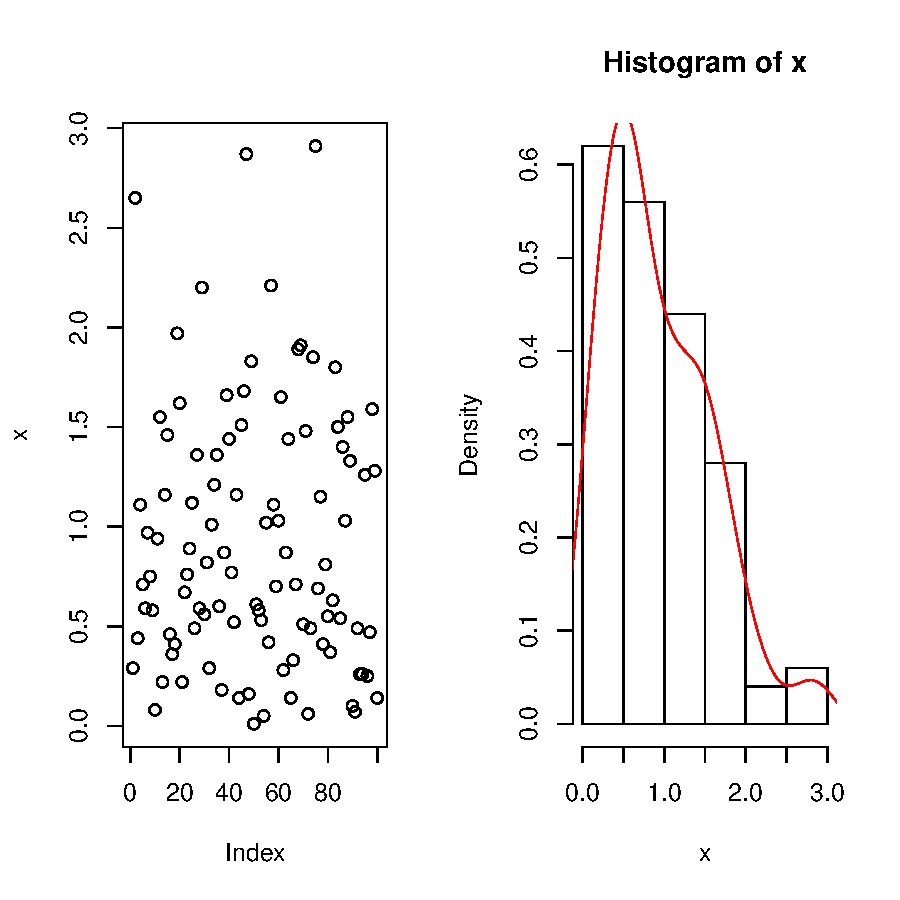
\includegraphics{outliers-001}

Above data simulated using normal distribution as it is clear from the plot. In code, \texttt{rnorm()} is used to simulate data sets from normal distribution. From the plot it is clear that the distribution is roughly normal. 

\subsubsection{Anomaly detection}

The following is the function for detecting anomalous data points. 

\begin{Schunk}
\begin{Sinput}
> outliers <- function(d, y = 90, o = "out"){
+   
+   if (!d){
+     d <- round(rnorm(100)*100, 2)
+   }
+   
+   c1 <- quantile(d, 0.75)
+   
+   if(y == 90){
+     ul <- mean(d) + 1.64*sd(d)
+     ll <- mean(d) - 1.64*sd(d)
+   
+   } else if(y == 95){
+     ul <- mean(d) + 1.96*sd(d)
+     ll <- mean(d) - 1.96*sd(d)
+   
+   }
+   
+   y <- matrix(NA, length(d), 1)
+   
+   for (i in 1:length(x)){
+     if (d[i] <= ll | d[i] >= ul){
+       y[i] <- d[i]
+     }
+   }
+   
+   plot(d, type = "l"); points(y, col = "red", pch = 19); abline(h=mean(d), col = "red");abline(h=ul, col = "green"); abline(h=ll, col = "green"); text(c1, ul, paste("UL=", round(ul, 2))); text(c1, ll, paste("LL=", round(ll, 2)))
+ 
+     if (o == "out"){
+     return(y[complete.cases(y)])
+   }
+ }
\end{Sinput}
\end{Schunk}

This creates UDF in R workspace. This function accepts two arguments one, data ditribution and second, confidence interval (ci), returns a plot with all outliers highlighted in red colour. 

\subsubsection{Testing}


\begin{Schunk}
\begin{Sinput}
> set.seed(123)
> x = rnorm(100)
> outliers(x, 95, o = "out")
\end{Sinput}
\begin{Soutput}
[1] -1.966617  2.168956  2.050085 -2.309169  2.187333
\end{Soutput}
\end{Schunk}
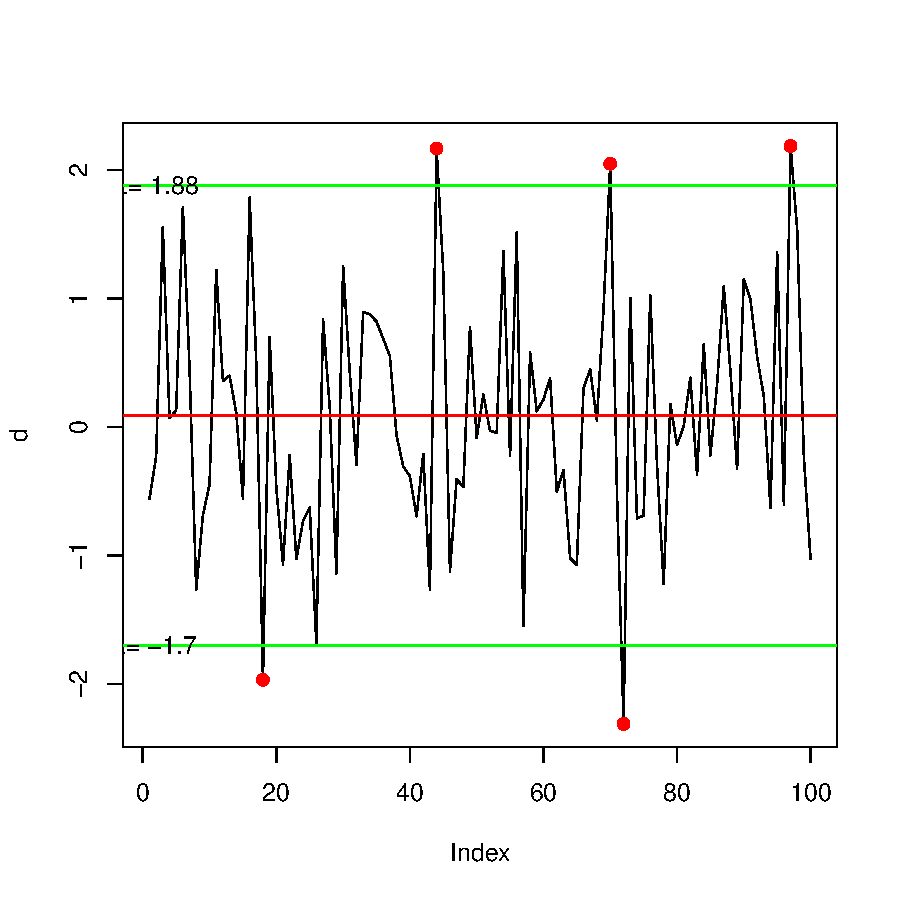
\includegraphics{outliers-003}

The points highlighted in red colour are \emph{outliers} but they are defined as outliers at 95 percent confidence interval. The green lines represents respective \emph{threshold limits}. Suppost if we define outliers at 90 percent confidence interval. The visual could be different with diferent number of data points. 

\begin{Schunk}
\begin{Sinput}
> par(mfrow=c(2, 1))
> outliers(x, 90); outliers(x, 95)
\end{Sinput}
\begin{Soutput}
[1]  1.715065  1.786913 -1.966617 -1.686693  2.168956 -1.548753  2.050085
[8] -2.309169  2.187333
\end{Soutput}
\begin{Soutput}
[1] -1.966617  2.168956  2.050085 -2.309169  2.187333
\end{Soutput}
\end{Schunk}
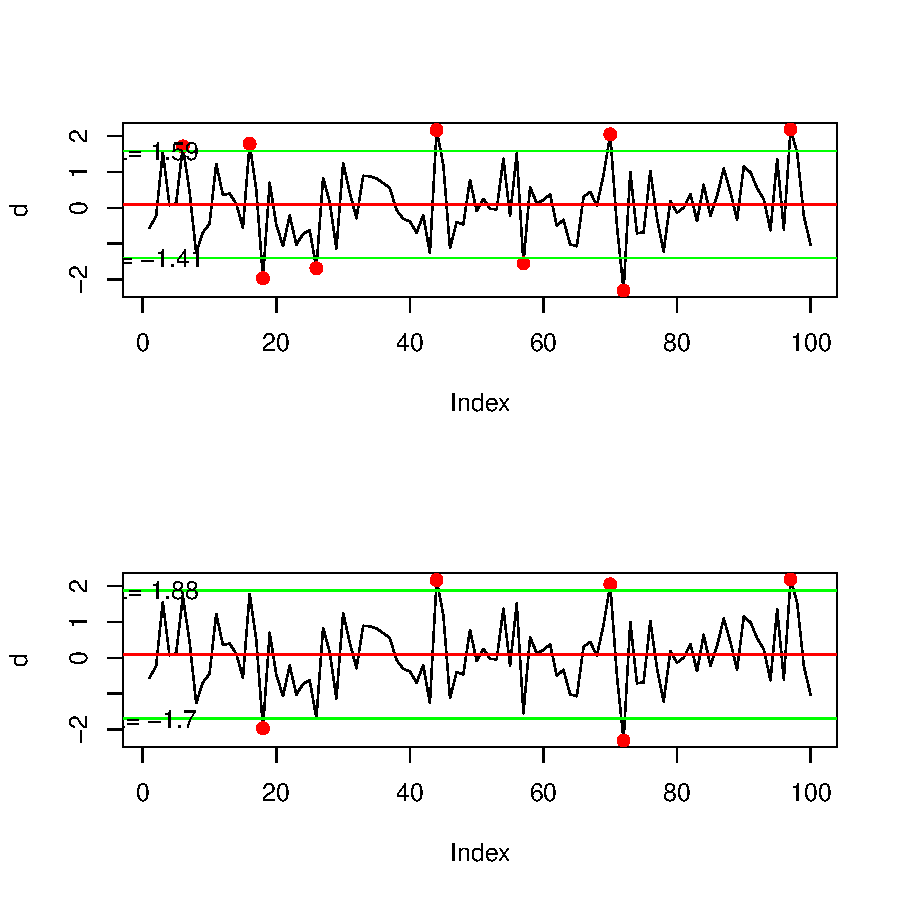
\includegraphics{outliers-004}

Plot above is the visual that has 90 percent of CI, while the below has data between 95 percent CI. Difference between number of outliers are clearly visible from the plot. 

\subsection{In Regression}

Linear models are highly commendable 

\begin{Schunk}
\begin{Sinput}
> fit <- lm(x ~ ., data = as.data.frame(x))
> cd <- cooks.distance(fit)
> plot(cd); abline(h = 4*mean(cd, na.rm = T), col ="red"); text(x = 1:length(cd)+1, y = cd, labels = ifelse(cd > 4*mean(cd, na.rm = T), names(cd), ""), col = "red")
\end{Sinput}
\end{Schunk}
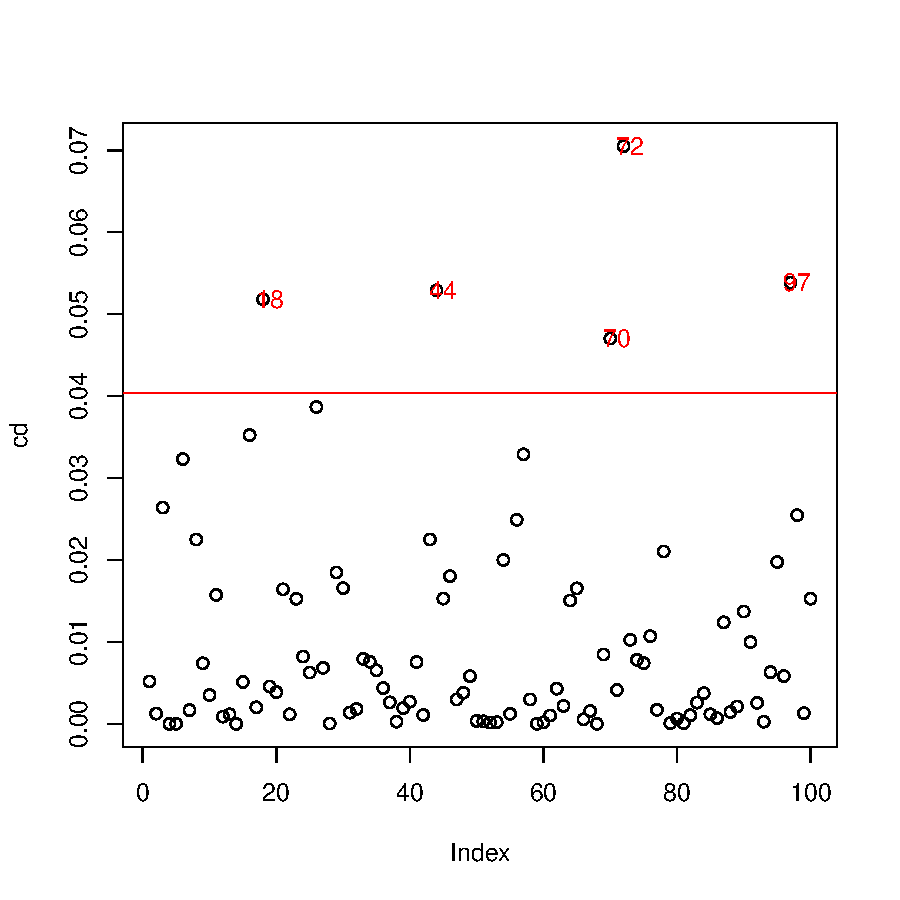
\includegraphics{outliers-005}





\end{document}
